\documentclass[12pt]{beamer}
\usepackage{../Estilos/BeamerMAF}
\usepackage[absolute, overlay]{textpos}
\usepackage{../Estilos/ColoresLatex}
\usetheme{Copenhagen}
\usecolortheme{wolverine}
%\useoutertheme{default}
\setbeamercovered{invisible}
% or whatever (possibly just delete it)
\setbeamertemplate{section in toc}[sections numbered]
\setbeamertemplate{subsection in toc}[subsections numbered]
\setbeamertemplate{subsection in toc}{\leavevmode\leftskip=3.2em\rlap{\hskip-2em\inserttocsectionnumber.\inserttocsubsectionnumber}\inserttocsubsection\par}
% \setbeamercolor{section in toc}{fg=blue}
% \setbeamercolor{subsection in toc}{fg=blue}
% \setbeamercolor{frametitle}{fg=blue}
\setbeamertemplate{caption}[numbered]

\setbeamertemplate{footline}
\beamertemplatenavigationsymbolsempty
\setbeamertemplate{headline}{}


\makeatletter
% \setbeamercolor{section in foot}{bg=gray!30, fg=black!90!orange}
% \setbeamercolor{subsection in foot}{bg=blue!30}
% \setbeamercolor{date in foot}{bg=black}
\setbeamertemplate{footline}
{
  \leavevmode%
  \hbox{%
  \begin{beamercolorbox}[wd=.333333\paperwidth,ht=2.25ex,dp=1ex,center]{section in foot}%
    \usebeamerfont{section in foot} \insertsection
  \end{beamercolorbox}%
  \begin{beamercolorbox}[wd=.333333\paperwidth,ht=2.25ex,dp=1ex,center]{subsection in foot}%
    \usebeamerfont{subsection in foot}  \insertsubsection
  \end{beamercolorbox}%
  \begin{beamercolorbox}[wd=.333333\paperwidth,ht=2.25ex,dp=1ex,right]{date in head/foot}%
    \usebeamerfont{date in head/foot} \insertshortdate{} \hspace*{2em}
    \insertframenumber{} / \inserttotalframenumber \hspace*{2ex} 
  \end{beamercolorbox}}%
  \vskip0pt%
}
\makeatother

\makeatletter
\patchcmd{\beamer@sectionintoc}{\vskip1.5em}{\vskip0.8em}{}{}
\makeatother

% %\newlength{\depthofsumsign}
% \setlength{\depthofsumsign}{\depthof{$\sum$}}
% \newcommand{\nsum}[1][1.4]{% only for \displaystyle
%     \mathop{%
%         \raisebox
%             {-#1\depthofsumsign+1\depthofsumsign}
%             {\scalebox
%                 {#1}
%                 {$\displaystyle\sum$}%
%             }
%     }
% }
% \def\scaleint#1{\vcenter{\hbox{\scaleto[3ex]{\displaystyle\int}{#1}}}}
% \def\scaleoint#1{\vcenter{\hbox{\scaleto[3ex]{\displaystyle\oint}{#1}}}}
% \def\bs{\mkern-12mu}


\setbeamercolor{section in foot}{bg=babyblue, fg=black}
\setbeamercolor{subsection in foot}{bg=blond, fg=black}

\makeatletter
\setbeamertemplate{footline}
{
\leavevmode%
\hbox{%
\begin{beamercolorbox}[wd=.333333\paperwidth,ht=2.25ex,dp=1ex,center]{section in foot}%
  \usebeamerfont{section in foot} \insertsection
\end{beamercolorbox}%
\begin{beamercolorbox}[wd=.333333\paperwidth,ht=2.25ex,dp=1ex,center]{subsection in foot}%
  \usebeamerfont{subsection in foot}  \insertsubsection
\end{beamercolorbox}%
\begin{beamercolorbox}[wd=.333333\paperwidth,ht=2.25ex,dp=1ex,right]{date in head/foot}%
  \usebeamerfont{date in head/foot} \insertshortdate{} \hspace*{1.5em}
  \insertframenumber{} / \inserttotalframenumber \hspace*{2ex} 
\end{beamercolorbox}}%
\vskip0pt%
}
\makeatother
\usefonttheme{serif}
\setbeamercolor{frametitle}{bg=champagne}
\resetcounteronoverlays{saveenumi}

\date{31 de mayo de 2022}

\title{\large{Tema 6 - Transformadas Integrales}}
\subtitle{Matemáticas Avanzadas de la Física}
\author{M. en C. Gustavo Contreras Mayén}

\begin{document}
\maketitle
\fontsize{14}{14}\selectfont
\spanishdecimal{.}

\section*{Contenido}
\frame{\frametitle{Temas a revisar} \tableofcontents[currentsection, hideallsubsections]}

\section{Transformadas integrales}
\frame{\tableofcontents[currentsection, hideothersubsections]}
\subsection{Introducción}

\begin{frame}
\frametitle{Registro y manejo de señales}
Una de las tareas generales de la física e ingeniería es registrar señales medidas y obtener información de ellas.
\\
\bigskip
\pause
Nos interesan principalmente las señales que varían con el tiempo.
\end{frame}
\begin{frame}
\frametitle{Tipos de señales}
Pueden ser señales periódicas o no periódicas, ruido o también superposiciones de componentes.
\\
\bigskip
\pause
De todos modos, lo que estamos midiendo es un conglomerado de varios componentes, lo que significa que los efectos causados por la electrónica de los dispositivos de medición y, por ejemplo, el ruido, se suman a la señal que realmente buscamos.
\end{frame}
\begin{frame}
\frametitle{Tipos de señales}
\begin{figure}
    \centering
    \only<1>{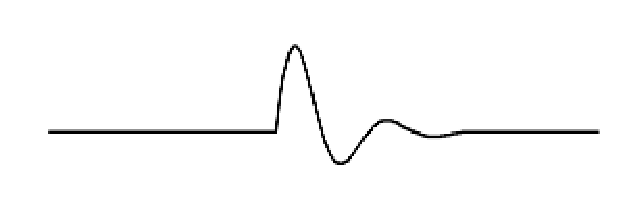
\includegraphics[scale=0.5]{Imagenes/TDF_01.eps}}
    \only<2>{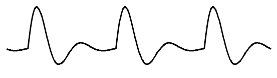
\includegraphics[scale=0.7]{Imagenes/TDF_02.png}}
    \only<3>{
\includegraphics[scale=0.7]{Imagenes/TDF_03.png}}
    \only<4>{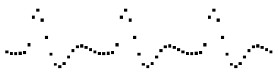
\includegraphics[scale=0.7]{Imagenes/TDF_04.png}}
\end{figure}
\end{frame}
\begin{frame}
\frametitle{Componentes de la señal}
Por eso tenemos que tomar la señal grabada, filtrar lo que nos interesa y procesarlo.
\\
\bigskip
\pause
En muchos casos estamos predominantemente interesados en los componentes periódicos de la señal, o el contenido espectral, que consta de componentes discretos.
\end{frame}
\begin{frame}
\frametitle{Utilidad de la transformada de Fourier}
Para análisis de este tipo, la transformada de Fourier es particularmente adecuada.
\end{frame}
\begin{frame}
\frametitle{Utilidad de la transformada de Fourier}
Aquí hay unos ejemplos:
\pause
\setbeamercolor{item projected}{bg=blue,fg=white}
\setbeamertemplate{enumerate items}{%
\usebeamercolor[bg]{item projected}%
\raisebox{1.5pt}{\colorbox{bg}{\color{fg}\footnotesize\insertenumlabel}}%
}
\begin{enumerate}[<+->]
\item Análisis de las vibraciones de una cuerda de violín o de un puente.
\item Comprobar la calidad de un amplificador de alta fidelidad.
\item Espectroscopia de TF de radiofrecuencia.
\item Espectroscopia óptica de TF.
\item Procesamiento digital de imágenes (bidimensionales y tridimensionales).
\end{enumerate}
\end{frame}
\begin{frame}
\frametitle{Algunos ejemplso}
Los anteriores solo son algunos ejemplos de acústica, electrónica y óptica.
\\
\bigskip
\pause
Lo que también demuestra que este método no solo es útil para la investigación puramente científica. \pause Muchos procedimientos matemáticos en casi todas las ramas de la física e la ingeniería utilizan la transformación de Fourier.
\end{frame}
\begin{frame}
\frametitle{El manejo conveniente de las transformadas}
El método es tan conocido, casi \enquote{viejo}, que los estudiantes/usuarios, a menudo solo tienen que presionar unos pocos botones (o usar unos pocos clicks del mouse) para realizar una transformada de Fourier.
\end{frame}
\begin{frame}
\frametitle{Desventaja de automatizar el cálculo}
Esta facilidad de uso, sin embargo, a menudo va acompañada de la pérdida de todos los conocimientos necesarios.
\\
\bigskip
\pause
Los errores de funcionamiento, las interpretaciones incorrectas y la frustración son el resultado de ajustes incorrectos o errores similares.
\end{frame}


\section{Objetivos}
\frame{\tableofcontents[currentsection, hideothersubsections]}
\subsection{Alcance del Tema 6}

\begin{frame}{Objetivos}
Al concluir el tema, se espera que el alumno:
\setbeamercolor{item projected}{bg=blue,fg=white}
\setbeamertemplate{enumerate items}{%
\usebeamercolor[bg]{item projected}%
\raisebox{1.5pt}{\colorbox{bg}{\color{fg}\footnotesize\insertenumlabel}}%
}
\begin{enumerate}[<+->]
\item Identifique la naturaleza de las transformadas integrales, así como los distintos tipos que existe en la física matemática.
\item Aplicará la transformada de Fourier para resolver distintos tipos de problemas con ecuaciones diferenciales parciales.
\seti
\end{enumerate}
\end{frame}
\begin{frame}{Objetivos}
\setbeamercolor{item projected}{bg=blue,fg=white}
\setbeamertemplate{enumerate items}{%
\usebeamercolor[bg]{item projected}%
\raisebox{1.5pt}{\colorbox{bg}{\color{fg}\footnotesize\insertenumlabel}}%
}
\begin{enumerate}[<+->]  
\conti
\item Reconocerá y utilizará la transformada de Laplace en ejercicios con ecuaciones diferenciales ordinarias y parciales.
\end{enumerate}
\end{frame}

\section{Contenido del Tema}
\frame{\tableofcontents[currentsection, hideothersubsections]}
\subsection{Introducción a las transformadas}

\begin{frame}
\frametitle{Introducción a las transformadas integrales}
Se revisará de manera general y con un punto de vista de aplicación, el concepto de transformada integral, así como los distintos tipos que se suelen encontrar en la Física Matemática.
\end{frame}
\begin{frame}
\frametitle{Introducción a las transformadas integrales}
Una vez revisada la definición de transformada integral, se presenta una lista con una serie de transformadas integrales, las de más uso en ciencia e ingeniería, así como transformadas especiales que se ocupan a partir de funciones especiales.
\\
\bigskip
\pause
Cada una de estas transformadas tiene su correspondiente transformada inversa.
\end{frame}

\subsection{La Transformada de Fourier}

\begin{frame}
\frametitle{La Transformada de Fourier}
Se hace una revisión sobre la Transformada de Fourier (TF) así como de la Transformada inversa de Fourier (TIF).
\\
\bigskip
\pause
Como herramienta necesaria se recomienda hacer una revisión sobre el tema de series de Fourier, ya que se ocuparán algunos resultados de ese tema.
\end{frame}
\begin{frame}
\frametitle{Propiedades de la TF}
Se discutirán una serie de propiedades de la Transformada de Fourier, en donde para algunos casos, se revisará la demostración de esas propiedades, dejando otras para revisión por parte del alumno, como tarea moral.
\\
\bigskip
\pause
Ocupando la definición de las transformadas es posible obtener el resultado, siguiendo una serie de pasos sencillos.
\end{frame}

\subsection{La Transformada de Laplace}

\begin{frame}
\frametitle{La Transformada de Laplace}
Se hace una revisión sobre la Transformada de Laplace (TL) así como la Transformada inversa de Laplace (TIL), destacando que esta transformada es la de mayor utilidad en física matemática.
\\
\bigskip
\pause
También se presentarán un conjunto de propiedades de la TL para ocuparla como herramienta de solución a problemas con ecuaciones diferenciales.
\end{frame}

\section{Cronograma}
\frame{\tableofcontents[currentsection, hideothersubsections]}
\subsection{Materiales de trabajo}

\begin{frame}
\frametitle{Lecturas de revisión}
Para lograr los objetivos del Tema 6, se tendrán que revisar los siguientes materiales de trabajo que estarán disponibles en la plataforma Moodle.
\\
\bigskip
\pause
\setbeamercolor{item projected}{bg=blue,fg=white}
\setbeamertemplate{enumerate items}{%
\usebeamercolor[bg]{item projected}%
\raisebox{1.5pt}{\colorbox{bg}{\color{fg}\footnotesize\insertenumlabel}}%
}
\begin{enumerate}[<+->]
\item Semana 15: Introducción a las transformadas integrales y Transformada de Fourier.
\item Semana 16: Transformada de Laplace.
\end{enumerate}
\end{frame}

\section{Evaluación}
\frame{\tableofcontents[currentsection, hideothersubsections]}
\subsection{Ejercicios semanales}

\begin{frame}
\frametitle{Ejercicios}
Dado el tiempo que se tiene para completar el último tema del curso, los ejercicios que se indicarán, \pause serán a modo de examen-tarea.
\\
\bigskip
\pause
La calificación obtenida será parte del segundo examen parcial del curso.
\end{frame}
\begin{frame}
\frametitle{Entrega de las actividades}
El plazo de las actividades se reduce en comparación con los plazos para los otros temas, \pause se tendrá solo un fin de semana para la entrega.
\\
\bigskip
\pause
La cantidad de ejercicios es menor para compensar el corto tiempo.
\end{frame}
\begin{frame}
\frametitle{Entrega de los ejercicios}
Se entregarán los ejercicios será vía Moodle a las 6 pm, de la siguiente manera:
\pause
\setbeamercolor{item projected}{bg=red,fg=white}
\setbeamertemplate{enumerate items}{%
\usebeamercolor[bg]{item projected}%
\raisebox{1.5pt}{\colorbox{bg}{\color{fg}\footnotesize\insertenumlabel}}%
}
\begin{enumerate}[<+->]
\item Transformada de Fourier: Martes 7 de junio.
\item Transformada de Laplace: Lunes 13 de junio.
\end{enumerate}
\end{frame}
\begin{frame}
\frametitle{Entrega de los ejercicios}
Los ejercicios de los subtemas se entregan en la sesión del Martes 31 de mayo.
\\
\bigskip
\pause
De manera que cuenten con la oportunidad de adelantar las soluciones y en caso de requerirlo, solicitar una orientación o aclaración de dudas.
\end{frame}

\section{Sesiones de trabajo}
\frame{\tableofcontents[currentsection, hideothersubsections]}
\subsection{Clases presenciales}

\begin{frame}
\frametitle{Actividades en clase}
De acuerdo al calendario de las últimas semanas, se tendrán las sesiones presenciales:
\setbeamercolor{item projected}{bg=buff,fg=black}
\setbeamertemplate{enumerate items}{%
\usebeamercolor[bg]{item projected}%
\raisebox{1.5pt}{\colorbox{bg}{\color{fg}\footnotesize\insertenumlabel}}%
}
\begin{enumerate}[<+->]
\item Martes 31 de mayo y jueves 2 de junio de 2022.
\item Martes 7 y jueves 9 de junio de 2022.
\item Martes 14 de junio, para revisión individual de calificaciones y revisar la situación académica.
\end{enumerate}
\end{frame}
\begin{frame}
\frametitle{Fechas para el examen final}
En caso de que se requiera presentar el examen final, la mecánica será la siguiente:
\pause
\setbeamercolor{item projected}{bg=babyblue,fg=black}
\setbeamertemplate{enumerate items}{%
\usebeamercolor[bg]{item projected}%
\raisebox{1.5pt}{\colorbox{bg}{\color{fg}\footnotesize\insertenumlabel}}%
}
\begin{enumerate}[<+->]
\item Primera vuelta: se entregará el miércoles 15 de junio, para que lo regresen el viernes 17 a las 3 pm.
\item El lunes 20 de junio se informará sobre la evaluación obtenida.
\seti
\end{enumerate}
\end{frame}
\begin{frame}
\frametitle{Fechas para el examen final}
\setbeamercolor{item projected}{bg=babyblue,fg=black}
\setbeamertemplate{enumerate items}{%
\usebeamercolor[bg]{item projected}%
\raisebox{1.5pt}{\colorbox{bg}{\color{fg}\footnotesize\insertenumlabel}}%
}
\begin{enumerate}[<+->]
\conti  
\item En caso de aplicar la segunda vuelta: el examen se entregará el lunes 20 de junio, para que lo regresen el miércoles 22 de junio a las 3 pm.
\item El jueves 23 de junio se informará sobre la evaluación obtenida.
\end{enumerate}
\end{frame}
\end{document}